% Section I: Introduction. Drafted from References/Artifact_discussions.md §I and
% References/comprehensive_report.md §I. Five subsections (A motivation, B
% computational asymmetry, C related work woven, D contributions, E notation +
% organization) per the plan at /home/vscode/.claude/plans/now-review-all-the-fluffy-cascade.md.

\subsection{Motivation}
\label{sec:intro:motivation}

\IEEEPARstart{T}rajectory planning for autonomous vehicles is a multi-objective optimization problem in which the operative constraints encode behavioural rules carrying distinct degrees of importance. A safety constraint --- avoidance of vulnerable road users (VRUs), avoidance of collisions with other vehicles --- must hold absolutely. A legal constraint --- obedience of speed limits, lane discipline, traffic-signal compliance --- should hold whenever safety permits. A comfort constraint --- bounded longitudinal and lateral acceleration --- should hold whenever the higher tiers allow. The \emph{rulebook} framework of Censi \emph{et al.}~\cite{censi2019liability} formalises this priority structure as a pre-order on rules, inducing a lexicographic order on the per-rule violation vectors. The trajectory selected by the planner is the one that minimises violations in priority order and then minimises a performance objective subject to those violations being held at their minima.

\begin{figure}[t]
    \centering
    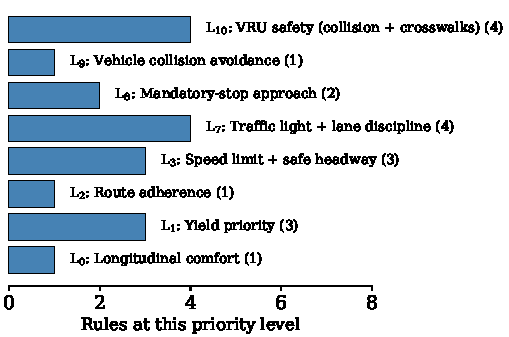
\includegraphics[width=\linewidth]{./Figures/fig01_g1_rulebook}
    \caption{Lexicographic priority structure of the 25-rule rulebook used by the LCP-MPC deployment. Rules are arranged by descending priority level, from vulnerable-road-user (VRU) collision at level $L_{10}$ to longitudinal and lateral comfort at level $L_0$. Each level groups one or more individually identified rules. Rule identifiers follow the convention $\langle\text{level}\rangle\mathtt{r}\langle\text{within-level index}\rangle$. The hierarchy is the empirical baseline against which the framework's lex-Pareto-dominance promise is assessed.}
    \label{fig:rulebook_hierarchy}
\end{figure}

Fig.~\ref{fig:rulebook_hierarchy} shows the rulebook hierarchy we adopt: a chain of priority levels from VRU safety ($L_{10}$) through longitudinal and lateral comfort ($L_0$). The rulebook is intentionally richer than what the convex framework of~\cite{lcp2025} can directly encode: of the 25 rules, 13 admit a convex per-step encoding (the MPC-controlled set), 9 are multi-tick state machines whose semantics fall outside the per-step template (the observer-only set), and 3 reserve OCP slot capacity for future enforcement but emit inactive constraints (the stub set). Section~\ref{sec:rulebook} formalises the $13 + 9 + 3 = 25$ partition; the comparative metric of Section~\ref{sec:protocol} operates only on the 13 MPC-controlled rules, with the 9 observer-only rules forming an invariant negative-control set.

\subsection{The Computational Asymmetry}
\label{sec:intro:asymmetry}

Two algorithmic strategies dominate the literature on priority-ordered constrained Model Predictive Control (MPC). The first, the \emph{lexicographic cascade}, solves a sequence of $L+1$ subproblems: at stage $i$, the violation functional $V_i$ is minimised over the optimal slice produced by stages $1, \ldots, i-1$, then the performance objective $J$ is minimised at stage $L+1$. The cascade is the exact realisation of the priority semantics but its computational cost is prohibitive at the $10$~Hz cadence used by closed-loop autonomous-vehicle simulators: each stage is a non-linear program warm-started from the previous stage's solution, and the per-stage iteration count grows monotonically as deeper stages enforce stricter active-set feasibility on top of all higher-priority slices. The empirical wall-time ratio is reported in Section~\ref{sec:results}~(\S\ref{sec:results:cost}); the operational consequence is that the cascade is unusable as the online planner and is reserved for offline reference and fallback.

The second strategy, \emph{weighted-sum scalarisation}, consolidates all priorities into a single objective
\begin{equation}
    \min_{z}\; J(z) + \sum_{i=1}^{L} w_i\, V_i(z),
    \label{eq:ws-scalarisation}
\end{equation}
with priority weights $w_1 \gg w_2 \gg \cdots \gg w_L > 0$. This is a single nonlinear program rather than $L+1$ sequential subproblems, giving an idealised solve-count reduction of factor $L+1$. The classical equivalent-weight result of Sherali~\cite{sherali1982equivalent} establishes that suitably chosen positive weights make the two formulations agree in linear programs; Eisenbrand, Niermann, and Skutella~\cite{eisenbrand2003lex} give explicit weight bounds for combinatorial cases. Charnes and Cooper~\cite{charnes1961goal} originated the goal-programming idiom in which such constructions naturally arise. In the convex MPC setting that dominates practical trajectory planning, the geometric structure of the equivalent-weight set has received less explicit attention; that gap is addressed by our foundation paper~\cite{lcp2025}, which characterises the equivalent-weight set as the unit-performance slice of the outward normal cone of the upper image of the achievement map.

The practitioner faces a recurring tension. The cascade is exact but slow; the scalarisation is fast but requires weights that one tunes empirically. Practitioners routinely observe that ``moderate weights work'' --- finite, non-astronomical weight separation produces solutions indistinguishable from the cascade --- but the geometric reason underlying this observation, and its operational consequences in a closed-loop autonomous-vehicle simulator, have not been validated end-to-end in the published literature. The present manuscript closes that validation gap.

\subsection{Related Work}
\label{sec:intro:related}

The present work draws on six lines of prior literature, which we group categorically.

\emph{Equivalent-weight theory.} The lineage from Charnes and Cooper~\cite{charnes1961goal} through Sherali~\cite{sherali1982equivalent} and Eisenbrand \emph{et al.}~\cite{eisenbrand2003lex} establishes the existence and computability of weights that make weighted-sum scalarisation recover the lexicographic optimum in linear and combinatorial programs. Our foundation paper~\cite{lcp2025} specialises this landscape to the convex MPC setting with a normal-cone presentation; the present manuscript validates the specialisation in deployment.

\emph{Prioritised constrained control.} Kanoun, Lamiraux, and Wieber~\cite{kanoun2011prioritized} developed prioritised inverse kinematics; Escande, Mansard, and Wieber~\cite{escande2014hqp} developed Hierarchical Quadratic Programming (HQP) for humanoid whole-body control. These approaches treat the cascade as the operational construct rather than seeking conditions under which it can be substituted by a single scalarised solve. The present deployment positions the calibrated weighted-sum planner as the operational mode and the cascade as the offline reference, inverting the operational primacy of the cascade.

\emph{Rulebook formalism for autonomous driving.} Censi \emph{et al.}~\cite{censi2019liability} established the rulebook as a pre-order on rules inducing lex on violation vectors. Esterle \emph{et al.}~\cite{esterle2020specification} treat behaviour specification with hierarchical guarantees. We work in the totally-ordered (chain) special case of the broader rulebook framework, which is sufficient for the rule set deployed by our planner.

\emph{Responsibility-sensitive safety (RSS) and IEEE 2846.} Shalev-Shwartz, Shammah, and Shashua~\cite{shalev2017rss} introduced RSS, pairing an instantly-checkable safety condition with a mathematically proven proper response so that compliance with the condition implies collision-free driving (\emph{assume-guarantee} on the other agents' behaviours). RSS is the basis of the IEEE 2846 standard~\cite{ieee2846}. Our framework occupies an adjacent niche: the per-level compliance vector $b_\epsilon$ provides runtime checks analogous to RSS conditions, but extended from RSS's binary blameless/blameworthy distinction to a continuous lex-priority structure over safety, legality, and comfort that admits graded trade-offs between levels.

\emph{Multi-objective optimisation and Pareto theory.} Wierzbicki~\cite{wierzbicki1980} developed the reference-point method; Yu~\cite{yu1985compromise} and Zeleny~\cite{zeleny1982compromise} developed compromise programming; Miettinen~\cite{miettinen1999nonlinear} provides the textbook treatment of multi-objective optimisation. Knee-point detection on the Pareto frontier~\cite{branke2004knee,das1999knee} provides operational tools for choosing among Pareto-optimal solutions. Our framework instead resolves the choice via the priority structure itself, with the equivalence region as the operationally relevant geometric object.

\emph{Sampling-based autonomous-vehicle planning.} Schwesinger \emph{et al.}~\cite{schwesinger2018sampling} developed sampling-based hierarchical motion planning. The present optimisation-based deployment offers continuous-action solutions with provable priority semantics at the cost of an offline calibration step.

\emph{Numerical methods and benchmarks.} The convex optimisation framework relies on the exact-penalty theory of Nocedal and Wright~\cite{nocedal2006numerical} and Bertsekas~\cite{bertsekas1999nonlinear} for the $L_1$/$L_2$ distinction. Implementations use IPOPT~\cite{wachter2006ipopt} via CasADi~\cite{andersson2019casadi}. The closed-loop simulator is nuPlan~\cite{caesar2021nuplan}, the public autonomous-driving benchmark released by Motional.

\subsection{Contributions}
\label{sec:intro:contributions}

Different from existing equivalent-weight literature~\cite{sherali1982equivalent,eisenbrand2003lex}, which establishes existence in linear and combinatorial settings, and different from prior prioritised-control work~\cite{escande2014hqp,kanoun2011prioritized}, which treats the cascade as the operational construct, in this work we build upon the geometric equivalence framework of~\cite{lcp2025} and present the following.

\begin{enumerate}
    \item \emph{A dynamics-agnostic reference implementation of the v10\_2 framework.} The \texttt{lcp} package implements Algorithm~0 (homogeneous-cone primary formulation, \cite{lcp2025} \S9.1), Algorithm~1A (box-bounded Chebyshev for the $L_1$ exact-equivalence regime, \cite{lcp2025} \S9.3), and Algorithm~1B (pointwise coupled-linear Chebyshev for the $L_2$ tolerance-compliance regime, \cite{lcp2025} \S9.4), together with the failure-mode pre-flight diagnostics of \cite{lcp2025} \S8.5, the online cascade-fallback + recalibration policy of \cite{lcp2025} \S9.6, the Relaxation Decision Framework of \cite{lcp2025} \S10, and the upper-image reification of \cite{lcp2025} \S3. The implementation reproduces the published numerical answers of the framework's worked examples to $10^{-6}$ precision via a 55-test regression suite (Appendix~\ref{app:verification}): for Example~1 (two-priority $L_1$ LP), $w^\dagger = (5.5, 5.5)$, $r^\dagger = 4.5$, and the equivalence region $\Omega(p^\star) = \{w_1 \ge 1, w_2 \ge 1\}$; for Example~2 (three-priority $L_2$ QP), the sensitivity constant $c_1 = 7$, the coupling $\kappa_1[3] = 0.75$, and the paper-published witness $(200, 100, 10)$ achieves threshold slack $5.5$.

    \item \emph{A closed-loop deployment on the nuPlan simulator that realises the calibrated weighted-sum substitution of \cite{lcp2025}'s formal lex cascade.} Closed-loop lexicographic-priority MPC has prior art in robotics (Hierarchical Quadratic Programming~\cite{escande2014hqp} on humanoids), and rule-based planners have been deployed on nuPlan before (notably \texttt{PDM-Closed}~\cite{dauner2023pdm}). The novelty here is the realisation of \cite{lcp2025}'s support-normal equivalence in closed loop on a kinematic-bicycle MPC, not the existence of a closed-loop priority planner. The deployment realises the framework as a two-level MPC pipeline (Section~\ref{sec:deployment}) and contributes eleven implementation primitives that the convex framework does not directly address but that the practical deployment had to invent: sequential linearisation for non-convex kinematic-bicycle dynamics; polygon-to-half-plane reduction for non-convex map disjunctions; per-tick applicability masking with a static slot budget; ego-local-frame solving with $L_1$ Tikhonov regularisation; a runtime compliance checker as the framework's online safety net; and a serialisation-tolerance contract for the CasADi solver state under nuPlan's planner-pickling pipeline.

    \item \emph{A 32-run dual-condition demonstration protocol on the 16-scenario \texttt{nuPlan-mini} benchmark} (Section~\ref{sec:protocol}). The two conditions are $C_1$ (the operational calibrated weighted-sum planner in $L_1$ mode) and $C_4$ (the formal lex cascade as the reference). The protocol is qualitative rather than statistical: with only $L+1$ priority levels per scenario, the structural property of interest --- whether the weighted-sum solve matches the cascade's priority-respecting compromise pattern --- is established by inspection of per-tick compliance vectors and per-level violation time series, not by hypothesis testing.

    \item \emph{Empirical demonstration that the calibrated weighted-sum planner produces priority-respecting compromise on every scenario in the benchmark.} For each scenario the per-level integrated violation breakdown (Fig.~\ref{fig:level_breakdown}) confirms that the low-priority levels $L_0$--$L_3$ absorb the compromise while the high-priority levels $L_8$--$L_{10}$ remain effectively held; the per-tick compliance match rate between $C_1$ and $C_4$ (Fig.~\ref{fig:compliance_match}) certifies that \cite{lcp2025}'s Theorem~4.1 holds in deployment at the effectively-held levels (median match rate $1.000$ at $L_{10}$ and $L_2$, $0.987$ at $L_9$, $0.981$ at $L_8$); the per-scenario wall-time ratio (Fig.~\ref{fig:walltime}) quantifies the operational benefit of the weighted-sum substitution over the cascade (median $6.22$, range $1.76$--$9.39$). The pre-flight diagnostics of \cite{lcp2025} \S8.5 (Table~\ref{tab:diagnostics}) and the empirical \S10.2 necessity scan (Table~\ref{tab:necessity}) tie the field behaviour back to the framework's standing assumptions.

    \item \emph{Eleven operational lessons for practitioners} (Table~\ref{tab:lessons_learned}, Section~\ref{sec:deployment}) consolidated as a roster: each primitive paired with the operational problem it solves, the failure symptom expected if absent, the workaround we chose, and the alternative we considered. The lessons-learned table is the practitioner-facing artefact of the deployment and the central contribution of Section~\ref{sec:discussion}.
\end{enumerate}

Our results suggest that the geometric equivalence framework of~\cite{lcp2025}, when augmented with the eleven deployment primitives reported here, is sufficient to realise priority-ordered constrained MPC on a closed-loop autonomous-vehicle simulator with both the operational throughput of weighted-sum scalarisation and the provable priority semantics of the formal lex cascade.

\subsection{Notation and Organisation}
\label{sec:intro:notation}

We use the notation of~\cite{lcp2025} throughout. State and control trajectories are denoted $z = (x_{0:N}, u_{0:N-1}) \in \mathbb{R}^d$; per-priority-level violation functionals are denoted $V_i$ for $i = 1, \ldots, L$; the performance objective is $J$. Per-tick decision variables include per-level slack matrices $T_i \in \mathbb{R}^{\text{slots}_i \times N}$ following the epigraph lift of~\cite{lcp2025}~\S5--\S7. Standard convex-analysis notation (outward normal cone $N_{\mathcal{S}}^{+}(p)$, subdifferential $\partial F$, relative interior $\mathrm{relint}(S)$) follows Rockafellar~\cite{rockafellar1970convex} and Boyd--Vandenberghe~\cite{boyd2004convex}.

The remainder of this manuscript is organised as follows. Section~\ref{sec:foundations} recaps the LCP framework from~\cite{lcp2025}, reproducing only what is load-bearing for the deployment and the empirical analysis. Section~\ref{sec:rulebook} presents the 25-rule rulebook and the $13 + 9 + 3 = 25$ partition that determines the index set over which the calibrated weighted-sum planner operates. Section~\ref{sec:deployment} describes the closed-loop deployment in detail through twelve subsections corresponding to the eleven implementation primitives plus the observer subsystem. Section~\ref{sec:protocol} formalises the dual-condition demonstration protocol and the empirical objects --- per-level integrated violation, per-tick compliance vector, per-scenario wall-time --- that the deployment is judged against. Section~\ref{sec:singlecondition} characterises the operational behaviour of the calibrated weighted-sum planner in isolation. Section~\ref{sec:results} reports the empirical evidence: the per-level violation breakdown demonstrating priority-respecting compromise, the $C_1$-vs-$C_4$ compliance match-rate as the operational realisation of Theorem~4.1, and the wall-time ratio quantifying the operational benefit of the weighted-sum substitution. Section~\ref{sec:discussion} discusses what the framework buys, its limitations, and its relationship to prior approaches. Section~\ref{sec:conclusion} concludes and outlines four directions of future work.
